\documentclass{article}
\usepackage[utf8]{inputenc}
\usepackage[T1]{fontenc}
\usepackage{graphicx}
\usepackage{hyperref}
\usepackage{geometry}
\geometry{margin=1in}

\title{THIROCE}
\date{Encyclopaedia Britannica (1771)}

\begin{document}
\maketitle

\section*{Historical source}
\textbf{Entry ID:} \texttt{entry-thiroce-604} \\
\textbf{Volume ID:} 193819047 \\
\textbf{Character Count:} 809

\subsection*{Extracted Text}
THIROCE, the ancient stone of a country in the S.E. of Europe, now forming part of European Turkey. In the earliest times the name was sent in a vastay seen, and applied to the whole region such of the Afghan Sen, including Macedonia and even Seythisu but with this morning become better known to the Greeky. Three was confined within narrower and more definite limits. It was bounded on the 7b, by the Danube, E. by the Exiton and the Boskolome, S. by the Proponits and the Aegean, and W. by the Strymon, or, as a later period by the Neustus, and the separated in from Macedonia. After the Roman conquest, its size was still further reduced by the chain of the same being made its northern boundary. It consenspala party with the modern Rumell, which also includes part of Macedonia and Thessaly. (See Rutuz)



\section*{Source record}
\begin{itemize}
\item \textbf{Dataset:} \texttt{NationalLibraryOfScotland/encyclopaedia\_britannica\_illustrated}
\item \textbf{Dataset Revision:} \texttt{309f765b1ecc83e0a7f7762e44b4a927a7555443}
\item \textbf{Page ID:} \texttt{britannica:309f765b1ecc83e0a7f7762e44b4a927a7555443:train:604} \\
  \textbf{Filename:} \texttt{page-0604-c50a825dd732.jpg} \\
  \textbf{Row Index:} 604 \\
  \textbf{SHA256:} \texttt{c50a825dd732a96e...}
\end{itemize}

\begin{figure}[h]
\centering
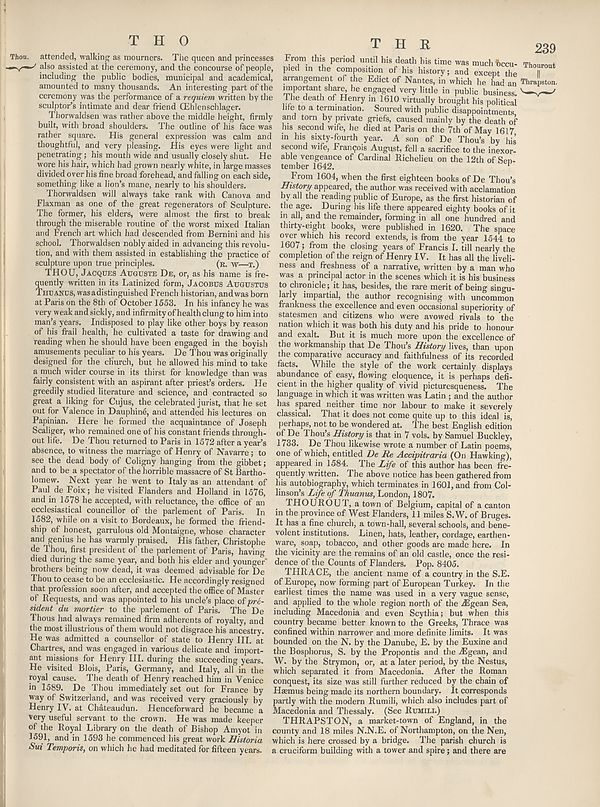
\includegraphics[width=0.85\textwidth]{../scans/page-0604-c50a825dd732.jpg}
\caption*{Source scan: \texttt{page-0604-c50a825dd732.jpg}}
\end{figure}

\end{document}
